\documentclass{article}
\usepackage{graphicx} % Required for inserting images
\usepackage{array}
\usepackage{multicol}
\usepackage[a4paper,margin=1.5cm]{geometry}

\newcolumntype{B}{>{\centering\arraybackslash}p{0.4cm}}

\title{Simple Accumulator Machine (SAM)}
\author{Stanley Lancaster}
\date{Feburary 2026}

% Start the document
\begin{document}

\maketitle
\pagebreak
\tableofcontents
\pagebreak

\section{Introduction}
The goal of this project is to implement a simple 16-bit accumulator machine in the style of the 16-bit minicomputers of the early 1970s. 
This is not designed to be a fast processor, nor is it designed to be an easy compiler target. 
Rather, it is designed to be easily implemented with TTL logic, and microcode.

\section {Block Diagram}
\begin{center}
    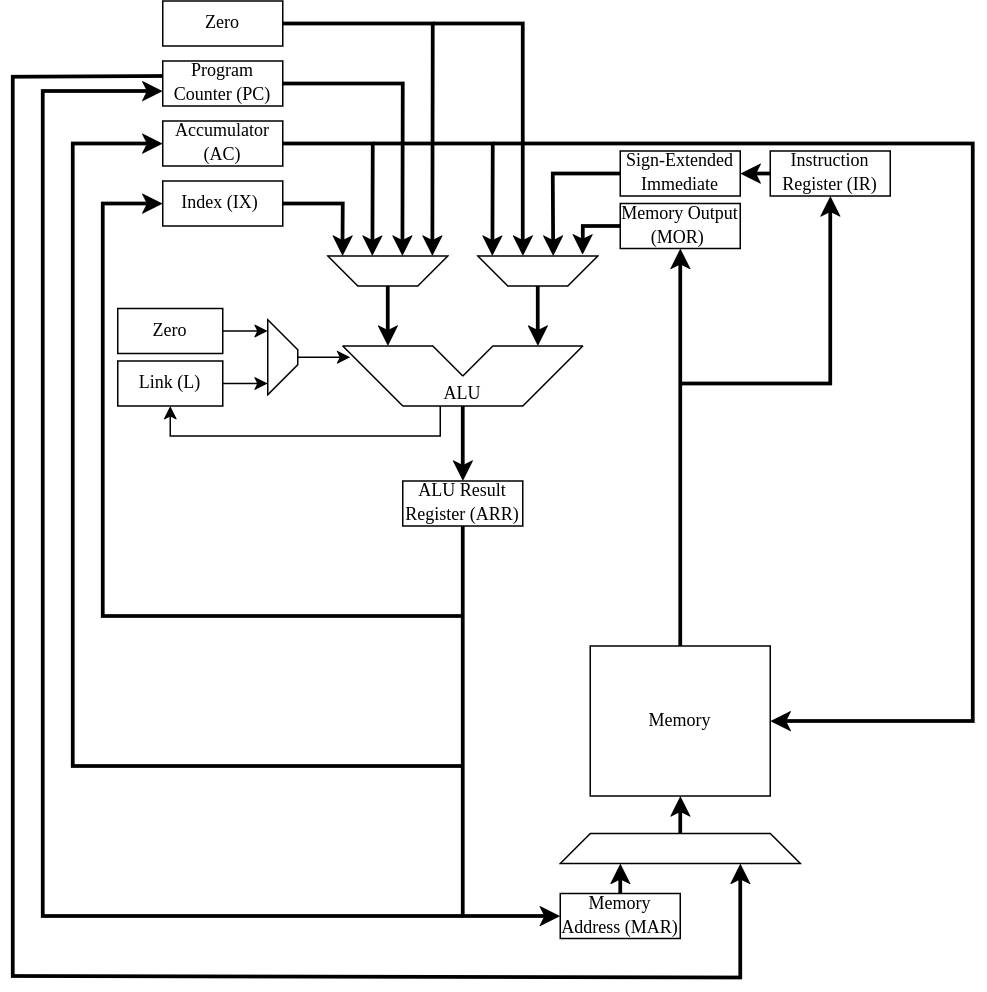
\includegraphics[scale=0.48]{BlockDiagram.png}
\end{center}

\pagebreak
\section{Instruction Set}
\begin{center}
\begin{tabular}{|c|c|c|c|c|c|c|c|c|c|c|c|c|c|c|c|c|}
    \hline
    ~ & \textbf{n0} & \textbf{n1} & \textbf{n2} & \textbf{n3} & \textbf{n4} & \textbf{n5} & \textbf{n6} & \textbf{n7} 
    & \textbf{n8} &  \textbf{n9} & \textbf{nA} & \textbf{nB} & \textbf{nC} & \textbf{nD} & \textbf{nE} & \textbf{nF} \\
    \hline
    \textbf{0n} & ~ & ~ & ~ & ~ & \verb|ld ac, IMM| & ~ & ~ & ~ & ~ & ~ & ~ & ~ & ~ & ~ & ~ & ~ \\
    \hline
    \textbf{1n} & ~ & ~ & ~ & ~ & ~ & ~ & ~ & ~ & ~ & ~ & ~ & ~ & ~ & ~ & ~ & ~ \\
    \hline
    \textbf{2n} & ~ & ~ & ~ & ~ & ~ & ~ & ~ & ~ & ~ & ~ & ~ & ~ & ~ & ~ & ~ & ~ \\
    \hline
    \textbf{3n} & ~ & ~ & ~ & ~ & ~ & ~ & ~ & ~ & ~ & ~ & ~ & ~ & ~ & ~ & ~ & ~ \\
    \hline
    \textbf{4n} & ~ & ~ & ~ & ~ & ~ & ~ & ~ & ~ & ~ & ~ & ~ & ~ & ~ & ~ & ~ & ~ \\
    \hline
    \textbf{5n} & ~ & ~ & ~ & ~ & ~ & ~ & ~ & ~ & ~ & ~ & ~ & ~ & ~ & ~ & ~ & ~ \\
    \hline
    \textbf{6n} & ~ & ~ & ~ & ~ & ~ & ~ & ~ & ~ & ~ & ~ & ~ & ~ & ~ & ~ & ~ & ~ \\
    \hline
    \textbf{7n} & ~ & ~ & ~ & ~ & ~ & ~ & ~ & ~ & ~ & ~ & ~ & ~ & ~ & ~ & ~ & ~ \\
    \hline
    \textbf{8n} & ~ & ~ & ~ & ~ & ~ & ~ & ~ & ~ & ~ & ~ & ~ & ~ & ~ & ~ & ~ & ~ \\
    \hline
    \textbf{9n} & ~ & ~ & ~ & ~ & ~ & ~ & ~ & ~ & ~ & ~ & ~ & ~ & ~ & ~ & ~ & ~ \\
    \hline
    \textbf{An} & ~ & ~ & ~ & ~ & ~ & ~ & ~ & ~ & ~ & ~ & ~ & ~ & ~ & ~ & ~ & ~ \\
    \hline
    \textbf{Bn} & ~ & ~ & ~ & ~ & ~ & ~ & ~ & ~ & ~ & ~ & ~ & ~ & ~ & ~ & ~ & ~ \\
    \hline
    \textbf{Cn} & ~ & ~ & ~ & ~ & ~ & ~ & ~ & ~ & ~ & ~ & ~ & ~ & ~ & ~ & ~ & ~ \\
    \hline
    \textbf{Dn} & ~ & ~ & ~ & ~ & ~ & ~ & ~ & ~ & ~ & ~ & ~ & ~ & ~ & ~ & ~ & ~ \\
    \hline
    \textbf{En} & ~ & ~ & ~ & ~ & ~ & ~ & ~ & ~ & ~ & ~ & ~ & ~ & ~ & ~ & ~ & ~ \\
    \hline
    \textbf{Fn} & ~ & ~ & ~ & ~ & ~ & ~ & ~ & ~ & ~ & ~ & ~ & ~ & ~ & ~ & ~ & ~ \\
    \hline
\end{tabular}
\end{center}

\pagebreak
\subsection{Add Immediate}
$DR \leftarrow SR + SignExtend(Immediate)$
\subsubsection{Description}
\begin{verbatim}
    addi DR, SR + Immediate   
    addi.c DR, SR + Immediate
\end{verbatim}
Add the sign extended immediate to the source register and place the result into the destination register. 
Update the link latch. 
If the condition bit (C) is set, and the link latch is not set, skip this instruction.

\subsubsection{Encoding}
\paragraph{\emph{Instruction Encoding}}
\renewcommand{\arraystretch}{1.5}
\begin{center}
    \begin{tabular}{|B|B|B|B|B|B|B|B|B|B|B|B|B|B|B|B|B|B|B|}
        \hline
        \textbf{15} & \textbf{14} & \textbf{13} &
        \textbf{12} & \textbf{11} & \textbf{10} & \textbf{9} &
        \textbf{8} & \textbf{7} & \textbf{6} & \textbf{5} &
        \textbf{4} & \textbf{3} & \textbf{2} & \textbf{1} &
        \textbf{0} \\

        \hline
        \multicolumn{1}{|c|}{0} & 
        \multicolumn{1}{c|}{0} & 
        \multicolumn{1}{c|}{0} & 
        \multicolumn{1}{c|}{C} & 
        \multicolumn{2}{c|}{DR} & 
        \multicolumn{2}{c|}{SR} & 
        \multicolumn{8}{c|}{Immediate} \\
        \hline
    \end{tabular}
\end{center}

\paragraph{\emph{Register Encoding}}
\begin{center}
    \begin{tabular}{|c|c|}
        \hline
        Register Name & Encoding \\
        \hline
        Zero & 00 \\
        \hline
        Accumulator (AC) & 01 \\
        \hline
        Index (IX) & 10 \\
        \hline
        Program Counter (PC) & 11 \\
        \hline
    \end{tabular}
\end{center}

\subsubsection{Associated Pseudo-Instructions}
\begin {center}
    \begin{tabular}{|c|c|c|}
        \hline
        Name & Syntax & Equivalent \\
        \hline
        Clear Link & cll & addi zero, zero + 0 \\
        \hline
        Set Link & stl & addi zero, zero - 1 \\
        \hline
        No-Operation & nop & addi.c zero, zero - 1 \\
        \hline
        Load immediate & ldi IMM & addi ac, zero + IMM \\
        \hline
        Clear Register & clr DR & addi DR, zero + 0 \\
        \hline
        Move & mov DR,SR & addi DR,SR + 0 \\
        \hline
        Increment & inc & addi ac,ac + 1  \\
        \hline
        Decrement & dec & addi ac,ac - 1 \\
        \hline
        Jump Relative & jr OFFSET & addi pc,pc + OFFSET \\
        \hline
        Jump Relative, Conditional & jr.c OFFSET & add.c pc,pc + OFFSET \\
        \hline
        Software Interrupt & int IMM & add pc, zero + IMM \\
        \hline
        Reset & rst & add pc, zero + 0 \\
        \hline
        Halt & hlt & addi pc,pc-1 \\
        \hline
    \end{tabular}
\end{center}

\pagebreak
\subsection{Arithmetic \& Logical Group}
$AC \leftarrow OP(SR, Memory[BASE + SignExtend(Immediate)])$
\subsubsection{Description}
\begin{verbatim}
    add SR, [BASE + Immediate]   
    sub SR, [BASE + Immediate]
    nor SR, [BASE + Immediate]
    eor SR, [BASE + Immediate]
\end{verbatim}
Apply the operation to the source register (SR) and the contents of the effective address ([BASE + Immediate]).
Deposit the result in the accumulator, and update the link latch.

\subsubsection{Encoding}
\paragraph{\emph{Instruction Encoding}}
\renewcommand{\arraystretch}{1.5}
\begin{center}
    \begin{tabular}{|B|B|B|B|B|B|B|B|B|B|B|B|B|B|B|B|B|B|B|}
        \hline
        \textbf{15} & \textbf{14} & \textbf{13} &
        \textbf{12} & \textbf{11} & \textbf{10} & \textbf{9} &
        \textbf{8} & \textbf{7} & \textbf{6} & \textbf{5} &
        \textbf{4} & \textbf{3} & \textbf{2} & \textbf{1} &
        \textbf{0} \\

        \hline
        \multicolumn{1}{|c|}{1} & 
        \multicolumn{1}{c|}{1} & 
        \multicolumn{2}{c|}{OP} &
        \multicolumn{1}{c|}{0} &
        \multicolumn{1}{c|}{SR} &
        \multicolumn{2}{c|}{BASE} & 
        \multicolumn{8}{c|}{Immediate} \\
        \hline
    \end{tabular}
\end{center}

\paragraph{\emph{Operation Encoding}}
\begin{center}
    \begin{tabular}{|c|c|}
        \hline
        Operation & Encoding \\
        \hline
        Addition (add) & 00 \\
        \hline
        Subtraction (sub) & 01 \\
        \hline
        Not-Or (nor) & 10 \\
        \hline
        Exclusive-Or (eor) & 11 \\
        \hline
    \end{tabular}
\end{center}

\paragraph{\emph{Source Register Encoding}}
\begin{center}
    \begin{tabular}{|c|c|}
        \hline
        Register Name & Encoding \\
        \hline
        Zero & 0 \\
        \hline
        Accumulator (AC) & 1 \\
        \hline
    \end{tabular}
\end{center}

\paragraph{\emph{Base Register Encoding}}
\begin{center}
    \begin{tabular}{|c|c|}
        \hline
        Register Name & Encoding \\
        \hline
        Zero & 00 \\
        \hline
        Accumulator (AC) & 01 \\
        \hline
        Index (IX) & 10 \\
        \hline
        Program Counter (PC) & 11 \\
        \hline
    \end{tabular}
\end{center}

\subsubsection{Associated Pseudo-Instructions}
\begin {center}
    \begin{tabular}{|c|c|c|}
        \hline
        Name & Syntax & Equivalent \\
        \hline
        Load Word & ld [BASE + IMM] & add zero, [BASE + IMM] \\
        \hline
        Invert & inv [BASE + IMM] & nor zero, [BASE + IMM] \\
        \hline
        Two's Complement & tc [BASE + IMM] & sub zero, [BASE + IMM] \\
        \hline
    \end{tabular}
\end {center}

\pagebreak
\subsection{Store}
$Memory[BASE + SignExtend(Immediate)] \leftarrow AC$
\subsubsection{Description}
\begin{verbatim}
    st [BASE + Immediate]
\end{verbatim}
Store the contents of the accumulator (AC) to memory at the address $BASE + SignExtend(Immediate)$

\subsubsection{Encoding}
\paragraph{\emph{Instruction Encoding}}
\renewcommand{\arraystretch}{1.5}
\begin{center}
    \begin{tabular}{|B|B|B|B|B|B|B|B|B|B|B|B|B|B|B|B|B|B|B|}
        \hline
        \textbf{15} & \textbf{14} & \textbf{13} &
        \textbf{12} & \textbf{11} & \textbf{10} & \textbf{9} &
        \textbf{8} & \textbf{7} & \textbf{6} & \textbf{5} &
        \textbf{4} & \textbf{3} & \textbf{2} & \textbf{1} &
        \textbf{0} \\

        \hline
        \multicolumn{1}{|c|}{1} & 
        \multicolumn{1}{c|}{0} & 
        \multicolumn{1}{c|}{0} &
        \multicolumn{1}{c|}{0} &
        \multicolumn{1}{c|}{0} &
        \multicolumn{1}{c|}{1} &
        \multicolumn{2}{c|}{BASE} & 
        \multicolumn{8}{c|}{Immediate} \\
        \hline
    \end{tabular}
\end{center}

\paragraph{\emph{Register Encoding}}
\begin{center}
    \begin{tabular}{|c|c|}
        \hline
        Register Name & Encoding \\
        \hline
        Zero & 00 \\
        \hline
        Accumulator (AC) & 01 \\
        \hline
        Index (IX) & 10 \\
        \hline
        Program Counter (PC) & 11 \\
        \hline
    \end{tabular}
\end{center}

\pagebreak
\section{Note About Absoloute Jumps}
NOTE: Should I have explicit call and return instructions. With space for stack adjustment, as well
as far calls?
\subsection{Far Jumps}
There is no simple pseudo instruction for absoloute `far' jumps, farther away than +/- 127 words.
In order to achieve this effect, the folling three-word sequence can be used.

\begin{verbatim}
    far_jump:
        ld [pc + address_label]
        mov pc, ac
    address_label:
        .word far_pointer
\end{verbatim}

\subsection{Far Calls}
Similar to far jumps, function calls can be complex. 
They require a far jump, as well as space to save the return pointer to the stack
\begin{verbatim}
    far_call:
        ld [pc + address_label]
        st [IX + 0]
        mov pc, ac
    address_label:
        .word far_call
        ; more code in this caller

    far_call:
        ; my function code
    return_now:
        ld [IX + 0]
        inc
        mov pc, ac
\end{verbatim}


\end{document}
